\documentclass[english, 12pt, a4paper, sci, a-1b, online]{aaltothesis}

\usepackage[numbers]{natbib}
\usepackage{graphicx}
\usepackage[most]{tcolorbox}
\usepackage{amsmath}
\usepackage{unicode-math}
\setmathfont{texgyrepagella-math.otf}

\usepackage{tkz-graph}
\usepackage{tikz}
\usetikzlibrary{calc}
\usetikzlibrary{arrows.meta}

\usepackage{minted}
\usemintedstyle{friendly}
\setmonofont{DejaVu Sans Mono}
\setminted{fontsize=\footnotesize}
% horrible hack to hide pygment's complaints about unicode
\AtBeginEnvironment{minted}{\dontdofcolorbox}
\def\dontdofcolorbox{\renewcommand\fcolorbox[4][]{##4}}

\degreeprogram{Computer, Communication and Information Sciences}
\major{Computer Science}
\code{SCI3042}

\univdegree{MSc}
\thesisauthor{Joonatan Saarhelo}
\thesistitle{Fast and Correct Round Elimination}
\place{Espoo}
\date{2021}

\supervisor{Prof.\ Jukka Suomela}
%\advisor{}

%% \uselogo{aaltoRed|aaltoBlue|aaltoYellow|aaltoGray|aaltoGrayScale}{?|!|''}
\uselogo{aaltoRed}{''}

\keywords{For keywords choose\spc{}concepts that are\spc{}central to your\spc{}thesis}

\thesisabstract{
Your abstract in English. Cannot contain special characters, linebreak or paragraph
break characters as it is written into the metadata.
}

%% Copyright text. Copyright of a work is with the creator/author of the work
%% regardless of whether the copyright mark is explicitly in the work or not.
%% You may, if you wish, publish your work under a Creative Commons license (see
%% creaticecommons.org), in which case the license text must be visible in the
%% work. Write here the copyright text you want. It is written into the metadata
%% of the pdf file as well.

\copyrighttext{Copyright \noexpand\copyright\ \number\year\ \ThesisAuthor}
{Copyright \textcopyright{} \number\year{} \ThesisAuthor}

\begin{document}

\makecoverpage{}

\makecopyrightpage{}

\begin{abstractpage}[english]
  \abstracttext{}
\end{abstractpage}

\newpage

\thesistitle{Nopea ja virheetön kierroseliminaatio}
\keywords{Vastus, resistanssi, lämpötila}

\begin{abstractpage}[finnish]
  Tiivistelmässä on lyhyt selvitys
  kirjoituksen tärkeimmästä sisällöstä: mitä ja miten on tutkittu,
  sekä mitä tuloksia on saatu. 
\end{abstractpage}

\thesistableofcontents{}


\mysection{Symbols and abbreviations}

\newcommand{\reline}[1]{\textbf{#1}}

\tikzstyle{active} = [draw, thick, circle, fill=white, minimum size=1.5em]
\tikzstyle{passive} = [draw, thick, circle, fill=darkgray, text=white, minimum size=1.5em]

\subsection*{Symbols}

\begin{tabular}{ll}
\end{tabular}

\subsection*{Abbreviations}

\begin{tabular}{ll}
RE         & round elimination
\end{tabular}

\cleardoublepage{}
\section{Introduction}

%% Leave page number of the first page empty
\thispagestyle{empty}

\clearpage
\section{History of computer-aided mathematics}

\section{Graph Theory}

\section{Locally Checkable Labeling}

Locally Checkable Labeling (LCL) is a family of graph coloring problems. In them, one has to assign colors to edges or vertices, satisfying some locally checkable condition.

Locally checkable means that a solution can be checked by checking fixed size neighborhoods. For example, to verify that vertices are properly colored, one just has to look at the neighbors of each vertex and check that no neighbor has the same color.

\subsection{Encoding for Round Elimination}

Round Elimination operates on a specific kind of edge coloring LCLs. They take place in \emph{biregular} graphs; which means graphs with properly two-colored vertices where the degree of each class of vertices is constant. One of the classes is called the active side and the other is the passive side.

Each side's vertices have their own rule that governs the combinations of colors neighboring edges are allowed to have. The rules can be written down by listing all allowed color combinations. Each allowed color combination is called a \emph{configuration}.

Most problems don't naturally give rise to this kind of LCL but have to be converted into it.

For example, take sinkless orientation. In that problem a direction must to be assigned to each edge, such that no vertex has only incoming edges.

\begin{figure}[h]
\centering
\begin{tikzpicture}[line width=1pt]
  \node [active] at (5, 0) (center') {};
  \node [active] at (0, 0) (center) {};
  \foreach \a/\cl/\el/\arrow in {0/O/I/-latex, 120/O/I/-latex, 240/I/O/latex-}
  {
    \node [active] at (\a+18:1.4) (A){};
    \draw [\arrow] (center) -- (A)
    coordinate[near start] (tail)
    coordinate[near end] (head);

    \node [passive] at ($ (\a+18:1.5) + (center') $) (P) {};
    \node [active] at ($ (\a+18:3) + (center') $) (A') {};
    \draw
    (center') -- (P) node[midway, fill=white] (CtoP) {\cl}
    (P) -- (A') node[midway, fill=white] (PtoA) {\el};
    \draw [dotted] \foreach \da in {-60, 60} {
      (A) -- ($ (A) + (\a+18+\da:0.8) $)
      (A') -- ($ (A') + (\a+18+\da:1) $)
    };
  };
  \draw [dashed, stealth-stealth, shorten <=0.6ex] (tail) to[bend left=10] (CtoP);
  \draw [dashed, stealth-stealth, shorten <=0.5ex] (head) to[bend left=10] (PtoA);
\end{tikzpicture}
\caption{Correspondence between solutions in round elimination graph and original graph}
\end{figure}

Each vertex in the original graph corresponds to an active vertex in the new one and edges correspond to passive vertices. We can describe the directions of edges by coloring them with I (for incoming) on O (for outgoing). The active side's rule follows from the problem description: all edges must not be incoming. The passive side's rule ensures that each edge is incoming on one end and outgoing on the other; otherwise there could be edges with an arrowhead on both sides.

\subsection{The LOCAL model}

This paper (and Round Elimination) is specifically about solving LCL-problems in the LOCAL model.

In the LOCAL model, each vertex runs the same program and must produce its own part of the solution. Each vertex can see its own unique id.

First, vertices get to compute as much as they need to. Then they send a message to each of their neighbors. All vertices receive the messages simultaneously. This process repeats until all vertices have chosen their output.

A problem for which there exists an algoritm that gives the correct output after $r$ rounds is called $r$-round solvable.

It can be shown that an $r$-round solvable problem is a problem where a correct output can be computed from the neighborhood of vertices up to $r$ edges away.


\section{Round Elimination}

Brandt et al.\ introduced round elimination in 2019\cite{speedup}. As the name suggests, it takes a problem $\Pi_0$ that can be solved in $r$ rounds and outputs a new problem $\Pi_1$ that is solvable in $r-1$ rounds. But what is $\Pi_1$ relationship to $\Pi_0$?

While $\Pi_0$ assigns a color to each edge, $\Pi_1$ assigns a set of colors each edge. That set contains the colors that the edge could have in a solution to $\Pi_0$. There is uncertainty because in $r-1$ rounds some information that affects the solution of $\Pi_0$ is out of reach.

\subsection{Lines}

Dennis Olivetti wrote an implementation of round elimination called Round Eliminator\cite{RE}. Round Elimination has been used to prove bounds on time complexity for various problems in the LOCAL model\cite{tc1, tc2, tc3}.

In Round Eliminator, problems are represented as \emph{lines}. Lines are a kind of shorthand notation that compresses multiple configurations into one line. Each line is a multiset of sets and represents or \emph{generates} all the configurations obtained by choosing one color from each set.\cite{RE}

For example, the line \reline{A BC} generates the configurations \reline{A B} and \reline{A C}.

\begin{figure}[h]
  \centering
  \begin{tcolorbox}[width=.2\textwidth, nobeforeafter, title=active side]
  A A A A \\
  B B B B \\
  C C C C
  \end{tcolorbox}
  \begin{tcolorbox}[width=.2\textwidth, nobeforeafter, title=passive side]
  A BC \\
  B C
  \end{tcolorbox}
  \caption{Three-coloring of a (4,2)-regular graph in Round Eliminator's shorthand}
\end{figure}

\subsection{Formal definition}
The configurations of $\Pi_1$ have the exact same shape as lines of $\Pi_0$: multisets of nonempty sets of symbols from $\Pi_0$'s alphabet, so it is convenient to talk about them as lines. I will call $\Pi_0$'s alphabet, active side and passive side $\Sigma_0$, $A_0$ and $P_{0}$ respectively and use the same notation to refer to $\Pi_{1}$'s components

The definition of RE from Distributed Algorithms 2020\cite{DA2020} rephrased in terms of lines:
\begin{itemize}
  \item $\Sigma_1$ is the powerset of $\Sigma_0$ minus the empty set.
  \item $A_{1}$ consists of all lines that only generate configurations present in $P_{0}$.
  \item $P_1$ consists of all lines that generate at least one configuration from $A_0$.
\end{itemize}

\subsection{Optimizing output size}

Round Elimination produces a gigantic number of configurations. Especially the new passive side contains almost every possible configuration. For example, suppose $\Sigma_{0} = {a, b, c}$ and $A_0$ has a configuration \reline{a~b}. Now $P_{1}$ contains \reline{a~b} but also \reline{ab~b}, \reline{ac~b}, \reline{abc~b}, \reline{a~ab}, \reline{a~bc}, \reline{a~abc}, \reline{ab~ab}, \reline{ab~bc}, \reline{ab~abc}, \reline{ac~ab}, \reline{ac~bc}, \reline{ac~abc}, \reline{abc~ab}, \reline{abc~bc} and \reline{abc~abc}. If we were to use this directly, the problem size would grow at an alarming rate with successive applications of round elimination, so it makes sense to optimize output size over round elimination speed.

One simple optimization is to discard all active configurations containing symbols that don't appear in any passive configurations and vice versa, as using them is impossible. But that isn't the only thing that can be done.

\subsubsection{Maximal form}

Suppose the picture below is part of a solution to $\Pi_{1}$. One can see that \reline{x~a} and \reline{af~y} are in $A_{1}$ and \reline{a~af} is in $P_{1}$. If \reline{x~ac} is in $A_{1}$, there is also a solution where node $n$ uses it instead of \reline{x~a}.

\begin{tikzpicture}[scale=2]
  \draw [thick, dashed] (0.3,0) -- (1,0) node[midway, above]{\{x\}};
  \draw [thick] (1,0) node[active]{n} -- (2, 0) node[midway, above]{\{a\}};
  \draw [thick, dashed] (3,0) -- (3.7,0) node[midway, above]{\{y\}};
  \draw [thick] (2,0) node[passive]{} -- (3, 0) node[active]{} node[midway, above]{\{a, f\}};
\end{tikzpicture}

In that alternative solution \reline{ac~af} has to be in $P_{1}$. \reline{a~af} is in $P_{1}$, so it generates some configuration from $A_{0}$. \reline{ac~af} generates strictly more configurations, so it is in $P_{1}$, too.

As every solution using \reline{x~a} can use \reline{x~ac} instead, \reline{x~a} can be omitted. In general, if two lines A and B can be ordered so that $\forall i : A_i \subseteq B_i$, A can be omitted.\cite{DA2020} For any A and B satisfying that criterion I say that B dominates A and A is dominated by B.

\tikzset{
  EdgeStyle/.append style = {->}
}
\begin{figure}[h]
  \centering
  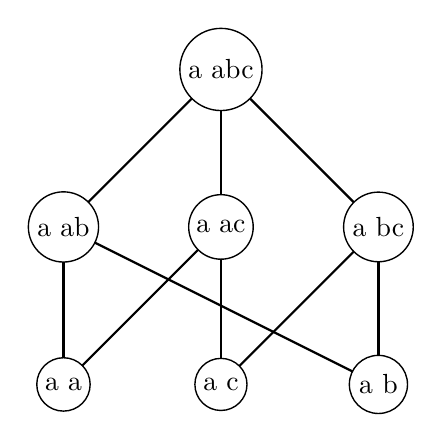
\begin{tikzpicture}
    \SetGraphUnit{2}
    \Vertex{a abc}
    \SO(a abc){a ac}
    \EA(a ac){a bc}
    \WE(a ac){a ab}
    \Edge(a abc)(a ac)
    \Edge(a abc)(a bc)
    \Edge(a abc)(a ab)
    \SO(a ac){a c}
    \EA(a c){a b}
    \WE(a c){a a}
    \Edge(a bc)(a b)
    \Edge(a bc)(a c)
    \Edge(a ac)(a c)
    \Edge(a ac)(a a)
    \Edge(a ab)(a a)
    \Edge(a ab)(a b)
  \end{tikzpicture}
  \caption{Graph of lines dominated by \reline{a~abc}.}
\end{figure}

Note that domination is not the same relation as $\text{configurations}(A) \subseteq \text{configurations}(B)$. \reline{a abc ade} generates \reline{a b e}, while \reline{a a bcde} only generates configurations that are in \reline{a abc ade}. Yet they are incomparable in terms of domination.

The subset of $A_{1}$ dominated by none is called the maximal form of $P_{0}$. Or one could say that the maximal form of $S$ is the Pareto front of \emph{valid} lines with respect to domination, where valid means that a line only generates configurations that $S$ generates.

This work's main contribution is a new algorithm for finding the maximal form of $P_{0}$ by combining lines and its proof.

% TODO explain proof that sets of configurations and lines are isomorphic

\subsection{Putting it all together}

To perform round elimination, one first finds the maximal form of the passive side. The new active side is a version of the maximal form where every set contains a single element, the corresponding set from the maximal form.

The new passive side is built simply by taking every line in the old active side and replacing the sets with all symbols from the new alphabet that contain the any of the old symbols.

Finally, to make the representation more compact, the symbols in the new alphabet are converted from subsets of the old alphabet to ordinals simply by enumerating the symbols.

\section{Coq Primer}

Before discussing my novel round elimination algorithm, I need to explain the basics of Coq because I will show the lemmas concerning its correctness as written in Coq's Vernacular. I will also give informal proofs. The actual proofs involve many boring details, which this paper does not cover. However, the Proving section will show examples of the most important proof techniques used. The full source code can be found in the project's repository\cite{source_code}.

\begin{listing}[h]
\begin{minted}{Coq}
Lemma tnth_zip n S T (a : n.-tuple T) (b : n.-tuple S) i :
  tnth (zip_tuple a b) i = (tnth a i, tnth b i).
\end{minted}
\caption{A very simple utility lemma which states that zipping two arrays of the same length and taking the $i$th item produces a tuple with the $i$th item of the first array and the $i$th item of the second list.}
\end{listing}

Lemmas in Coq are types. Constructing any value of type T proves the lemma T.

You are allowed to use values in types in order to make talking about computation convenient. This is called dependent types. Coq solves this with cumulative universes.


\section{Maximization via line combination}

In this section I'll present a maximization algorithm based on combining lines and the lemmas that I used to prove its correctness. I'll show the most important lemmas as they are written in Coq but present the proofs informally. The Proving section contains information on how the mechanized proofs were developed.

\newcommand\icoq[1]{\mintinline{Coq}{#1}}

\begin{listing}[h]
\begin{minted}{Coq}
Variable alphabet_size: nat.
Definition color := 'I_alphabet_size.
Variable one_minus_delta: nat.
Definition Δ := one_minus_delta.+1.

Definition nline n := n.-tuple {set color}.
Notation "n .-line" := (nline n) (at level 30, no associativity).
Definition line := Δ.-line.
Definition configuration := Δ.-tuple color.
\end{minted}
\caption{Definition of lines and configurations used throughout the proof.}
\end{listing}

Variables like \icoq{alphabet_size} automatically become arguments of any function that uses them in Coq. They are very convenient here, as I'd otherwise have to explicitly make many lemmas depend on the alphabet size and $\Delta$.

I use \icoq{one_minus_delta} to ensure that $\Delta$ is positive. That way I don't need to deal with the uninteresting case where vertices aren't connected at all. I could instead add \icoq{Variable nonzero_delta := Δ <> 0} but then I'd have to explicitly use it every time to eliminate the zero case.

\begin{listing}[h]
\begin{minted}{Coq}
Definition contains_unpermuted (cl: configuration) (l: line) : bool :=
  all2 (λ c (s : {set color}), c \in s) cl l.

Definition contains (cl : configuration) (line : line) : bool :=
  [exists (p : configuration | perm_eq p cl), contains_unpermuted p line].

Notation "a ∈ L" := (contains a L) (at level 50, no associativity).
\end{minted}
\caption{Lines are represented as tuples, so their lack of order is simulated, typically by operating on some permutation instead of the actual line.}
\end{listing}

\subsection{Combining lines}

My new maximization algorithm mostly consists of combining lines. Two lines can be combined by pairing up their sets and taking the union of one pair and the intersection of the rest.

\begin{minted}{Coq}
Definition combine m (n := m.+1) (a : n.-line) (b : n.-line) : n.-line :=
  [tuple of (thead a) :|: (thead b)
  :: map (λ ab, ab.1 :&: ab.2) (zip (behead a) (behead b))
  ].

Definition combination_of (a b c : line) :=
  ∃ (a' b' c' : line),
    perm_eq a' a ∧ perm_eq b' b ∧ perm_eq c' c ∧ combine a' b' = c'.

Theorem combination_is_sound (a b c : line) col :
  combination_of a b c -> col ∈ c -> col ∈ a ∨ col ∈ b.
\end{minted}

Proof: For each configuration \icoq{col} in \icoq{c}, wlog. suppose the symbol that comes from the union is from \icoq{a}. The symbols that come from intersections are in both \icoq{a} and \icoq{b}. Thus all symbols in \icoq{c} are from \icoq{a}.

\subsection{Domination relation}

\begin{minted}{Coq}
Definition dominates {n} (b a : n.-line) :=
  [exists a' : n.-line, exists b' : n.-line, perm_eq a a' && perm_eq b b' &&
    all2 (λ x y : {set color}, x \subset y) a' b'].
Notation "a ⊆ b" := (dominates b a) (at level 50, no associativity).
Notation "a ⊈ b" := (~~ dominates b a) (at level 50, no associativity).
Definition strictly_dominates {n} (b a : n.-line) := (a ⊆ b) && (b ⊈ a).
Notation "a ⊂ b" := (strictly_dominates b a) (at level 50, no associativity).
\end{minted}

The strict version of the domination relation is well-founded.

\begin{minted}{Coq}
Definition strictly_dominated (a b : line) := strictly_dominates b a.

Lemma strictly_dominated_wf : well_founded strictly_dominated.
\end{minted}

Proof: To show well-foundedness, one has to show that one always arrives a a smallest element by repeatedly picking any smaller element.

Define the weight of a line as the sum of its sets' cardinalities. Obviously no line can have a negative weight. If a line $a$ strictly dominates line $b$, then the weight of $b$ is smaller than the weight of $a$, since all of $b$'s sets are subsets of $a$'s and one is a strict subset.

There cannot be an infinite descending chain, as weight decreases while descending and weight is a natural number. QED.

\subsection{Finding the maximal form}

Any valid line can either be built by combining input lines or a line dominating it can be built. Thus the maximal lines can be built this way. The proof of this is less trivial and will be discussed later.

But even if combining lines eventually produces the maximal lines, that doesn't mean it is an efficient way of finding them. However, it can be shown that if combining a set of lines produces a line that isn't dominated by it, then two of the lines can be combined to produce some line that isn't dominated by any of them. In other words, we can make progress by simply trying all combinations of two lines!

\section{Performance}

Maximization is the most expensive part of the original Round Eliminator's algorithm. Maximization via line combination is orders of magnitude faster in practice and is resistant to some pathological inputs but it remains the most computationally expensive part. % TODO add to abstract maybe?

\subsection{Prior art}

The maximization algorithm previously used in Round Eliminator computes the set of invalid configurations by filtering all $|\Sigma|^{\Delta}$ possible configurations.

If every configuration was allowed, the maximal form would simply be a line that generates every configuration. The old algorithm starts with a list containing just that line. It then goes through all the invalid configurations, replacing every line in its list with narrowed down lines that don't generate that configuration.

The algorithm considers all permutations separately, so it produces $\Delta!$ copies of the output lines before deduplication.

% TODO continue this

Jukka Suomela pointed out an adversarial input that defeats this algorithm. Just concatenate multiple copies of an input, renamed so that each has its own disjoint subset of the alphabet. Then the number of valid lines grows linearly with the size of the input but the number of invalid configurations grows to the power of the degree.

\subsection{Output size}

If maximization could arbitrarily increase the number of lines, talking about worst-case performance would be of little practical use since any algorithmic inefficiency would be overshadowed by the size of the output. Thus it makes sense to find an upper bound for the size of the output.

The new lines found do not increase the number of configurations covered.

\subsection{Line combination}

The new algorithm's runtime doesn't depend on the size of the alphabet.

is approximately $O(n^{3}\Delta!)$.

The earlier algorithm computed all permutations of the maximal lines making the factorial unavoidable. It can be avoided in the new algorithm by using a smarter way to generate all combinations of two lines than presented here.


\section{Proving}

\subsection{Classical vs Intuitionistic Logic}

In Coq it is customary not to assume the law of excluded middle $\forall a : a \lor \lnot a$. This has little effect on the proof at hand, as it is about finite objects. For those a = b is equivalent to a == b and the latter is always true or false, as it can be computed.

\clearpage
\thesisbibliography{}

\bibliographystyle{plainnat}
\bibliography{correct_round_elimination}

%% Appendices
%% If you don't have appendices, remove \clearpage and \thesisappendix below.
\clearpage
\thesisappendix{}

\section{Esimerkki liitteestä\label{LiiteA}}

Kaavojen numerointi muodostaa liitteissä oman kokonaisuutensa:
\begin{align}
d \wedge A &= F, \label{liitekaava1}\\
d \wedge F &= 0. \label{liitekaava2}
\end{align}

\end{document}
